\chapter{Processo di Sviluppo}

\section{Gestione di Progetto}
Si è utilizzato \textit{Git} come sistema di DVCS del codice durante lo sviluppo, attraverso la piattaforma GitHub. L'abbiamo utilizzato sfruttando la tecnica del \textit{GitFlow} come mostrato nella figura \ref{pic:workflow}: il branch di default è sempre il \textit{main}, al quale \textit{development} è sempre allineato. Ogni volta che è necessario implementare una nuova \textit{feature} viene creato un branch da \textit{development}. Nel caso in cui debbano essere prodotti degli hotfix o risolti dei bug, essi vengono effettuati su un branch che parte da \textit{development} e vi ritorna, prima di essere mergiato nuovamente su \textit{main}. Successivamente, a lavoro ultimato, veniva creata una pull request per mergiare sul branch \textit{development} e infine sul \textit{main}.

\begin{figure}[ht]
    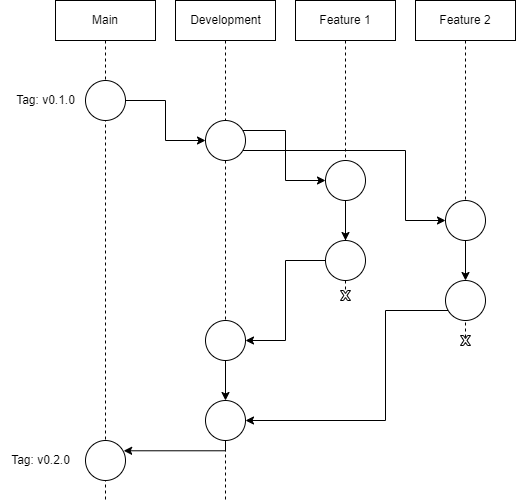
\includegraphics[width=9cm]{gitWorkflow.png}
    \centering
    \caption{\label{pic:workflow}Workflow del progetto.}
\end{figure}

\subsection{Versioning}
Il versioning è una scelta importante nello sviluppo di un progetto, perchè permette di dare un identificativo univoco ad una determinata versione del software.
\newline \newline Nella scelta della tipologia di sistema di versioning, il fattore che ha pesato di più è la frequenza di commit/modifiche del codice durante l'intero sviluppo della applicazione. Ci siamo da subito aspettati, infatti, che nella prima parte di progetto i commit sul nostro DVCS fossero più frequenti rispetto a quelli nella fase avanzata del progetto.
\newline \newline Abbiamo deciso quindi di adottare la tecnica del Semantic Versioning (\href{https://semver.org/lang/it/}{SEMVER}) che permette di capire, di versione in versione, quanto è effettivamente cambiato il codice, senza essere condizionato dalla frequenza di rilascio. 
Il semantic versioning è anche facilmente integrabile con il DVCS. \newline \newline Ogni numero di release rispetta il pattern \texttt{MAJOR.MINOR.PATCH}, in cui ad ogni release viene incrementato in base alle modifiche effettuate:
\begin{itemize}
    \item \texttt{MAJOR}: quando viene modificata l'API in maniera non retrocompatibile;
    \item \texttt{MINOR}: quando viene aggiunta una funzionalità in maniera retrocompatibile;
    \item \texttt{PATCH}: quando viene corretto un bug in maniera retrocompatibile.
\end{itemize}

Nel semantic versioning, vige inoltre la politica del no-retract, pertanto i numeri di versione sono sempre incrementali e non è possibile creare una release con versione precedente ad una già rilasciata, questo al fine di garantire maggior chiarezza e sapendo che a numero di versione più alto corrisponde la versione più recente.
\newline
\newline
Nel nostro progetto la scelta del numero di versione è stata lasciata agli sviluppatori. Ogni volta che viene fatta la push sul DVCS di un tag in formato \texttt{vMAJOR.MINOR.PATCH}, in automatico tramite un apposito workflow viene creata una release con allegati i compilati delle applicazioni e la documentazione aggiornata.

\subsection{Licensing}
Sono state considerate le principali licenze esistenti per progetti \textit{open-source} consultabili al seguente \href{https://choosealicense.com/licenses/}{\textit{link}}. \\
\newline La scelta è ricaduta sulla licenza di tipo GNU GPLv3 (GNU GENERAL PUBLIC LICENSE Version 3, 29 June 2007).
Questo tipo di licenza fa si che il nostro software possa essere utilizzato da altri autori purché questi pubblichino il proprio software con una licenza compatibile.

\section{Build Automation e continuos integration}

\subsection{Panoramica}
La build automation è stata realizzata utilizzando il servizio delle GitHub Actions. Tutti i \textit{job} implementati vengono eseguiti sui branch \textit{main} e \textit{development} ad ogni commit, pull-request e al push di un tag. Vengono descritti tutti i \textit{job} realizzati che vengono eseguiti sui diversi \textit{workflow} previsti:

\begin{itemize}
    \item \textbf{build-and-deploy-app-function}: utilizzato per deployare le \textit{Azure Function} di Azure;
    
    \item \textbf{build-simulator}: utilizzato per eseguire la build del simulatore e creare il rispettivo \textit{artifact};
    
    \item \textbf{build-client}: utilizzato per eseguire la build del client (lato simulatore) e creare il rispettivo \textit{artifact};
    
    \item \textbf{build-report}: utilizzato per compilare la relazione in Latex e creare l'\textit{artifact} relativo al file \texttt{.pdf};
    
    \item \textbf{execute-tests}: utilizzato per eseguire i test implementati;
    
    \item \textbf{release}: utilizzato per caricare gli artifacts nelle releases e per creare le versioni del progetto.
    
\end{itemize}

Inoltre sono stati implementati ulteriori due \textit{job} con lo scopo di notificarci se la build automation è terminata con successo o con un fallimento. La notifica si basa nel inviare un messaggio su un bot Telegram realizzato appositamente per il progetto (accessibile tramite questo \href{https://telegram.me/AzureHealthcareNotificator_bot}{\textit{link}}). Questi \textit{job} sono stati utilizzati nel workflow del branch \textit{development} e \textit{master}.
\begin{itemize}
    \item \textbf{jobs-failure}: notifica tramite un messaggio sul bot Telegram che la build è fallita;  
    
    \item \textbf{jobs-success}: notifica tramite un messaggio sul bot Telegram che la build è completata con successo.  
\end{itemize}

L'immagine \ref{pic:job-workflow} illustra il workflow descritto.

\begin{figure}[ht]
    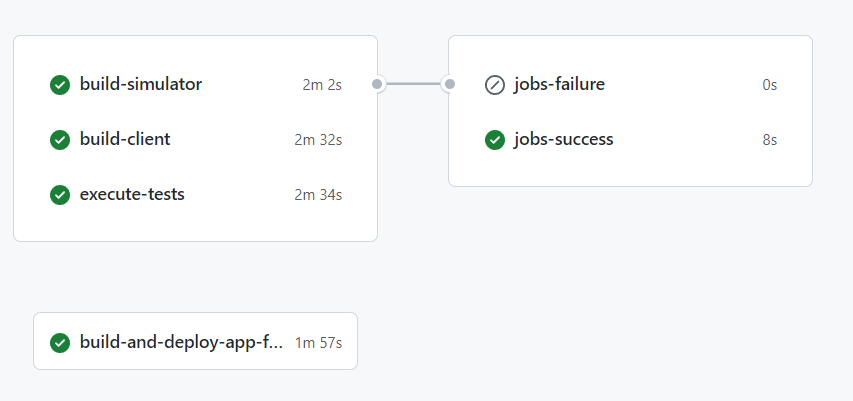
\includegraphics[width=12cm]{jobWorkflow.png}
    \centering
    \caption{\label{pic:job-workflow}Workflow dei job implementati.}
\end{figure}

\subsection{Relazione}
La relazione è stata scritta in Latex utilizzando l'editor  \href{https://it.overleaf.com/}{\textit{Overleaf}}. L'idea era quella di poter sincronizzare \textit{Overleaf} con il repository del progetto di \textit{GitHub} così che ad ogni modifica sull'editor corrispondeva un commit sul repository. Purtroppo questa è una funzionalità Premium che \textit{Overleaf} mette a disposizione e che non abbiamo potuto sfruttare. Oltre alla relazione in \texttt{.pdf} abbiamo realizzato anche quella web tramite le \href{https://pages.github.com/}{\textit{GitHub Pages}} consultabile al seguente \href{https://lucagiorgettismp.github.io/AzureHealthcareDigitalTwins/}{\textit{link}}.

\subsection{Test}
I test del progetto si sono concentrati sulla parte di generazione dei valori del simulatore. Non sono stati effettuati test né per la parte relativa ad Azure né per quella legata alla mixed reality. Questo perché nel primo caso, si tratta di un'infrastruttura cloud che non dispone di strumenti per effettuare i test mentre per la parte legata alla mixed reality, la motivazione è data dal troppo tempo richiesto per approfondire questa tematica in contesti come il nostro. \newline \newline Si è utilizzato il framework \textit{Visual Studio Unit Testing} con la quale ci ha permesso di testare:
\begin{itemize}
    \item la generazione dei valori dei sensori rispetto al valore minimo e massimo che questi possono raggiungere e ai propri valori di delta. In particolare, ogni nuovo valore di un determinato sensore da generare, deve ricadere in un range di $\mypm$ delta calcolato a partire dal vecchio valore di quel sensore;
    
    \item il corretto funzionamento dell'allarme se un valore appartiene (o meno) ad un range per descrivere se tale valore è nella norma o in una situazione di pericolo;
    
    \item la corretta generazione decrescente dei valori della batteria;
\end{itemize}

\subsection{Quality Assurance}
Per quanto riguarda la parte di qualità del codice, la scelta è ricaduta sui servizi \href{https://www.codefactor.io/}{\textit{Codefactor}} e \href{https://deepsource.io/}{\textit{DeepSource}}. \newline \par{CodeFactor} permette di essere facilmente integrabile a repository pubblici di Git Hub analizzando la qualità sintattica del codice. In questo modo ci ha permesso di correggere piccole imprecisioni e di conseguenza aumentarne la qualità. \newline \newline Un altro tool molto utile è DeepSource. Questo strumento permette di eseguire l'analisi semantica del codice, consentendo loro di rilevare diversi problemi, inclusi anti-pattern o rischi di bug in fase di esecuzione dell'applicativo.

